% Options for packages loaded elsewhere
\PassOptionsToPackage{unicode}{hyperref}
\PassOptionsToPackage{hyphens}{url}
%
\documentclass[
  11pt,
  a4paper,
]{article}
\usepackage{amsmath,amssymb}
\usepackage{iftex}
\ifPDFTeX
  \usepackage[T1]{fontenc}
  \usepackage[utf8]{inputenc}
  \usepackage{textcomp} % provide euro and other symbols
\else % if luatex or xetex
  \usepackage{unicode-math} % this also loads fontspec
  \defaultfontfeatures{Scale=MatchLowercase}
  \defaultfontfeatures[\rmfamily]{Ligatures=TeX,Scale=1}
\fi
\usepackage{lmodern}
\ifPDFTeX\else
  % xetex/luatex font selection
  \setmainfont[]{Noto Sans CJK JP}
  \setsansfont[]{Noto Sans CJK JP}
  \setmonofont[]{Noto Sans Mono CJK JP}
\fi
% Use upquote if available, for straight quotes in verbatim environments
\IfFileExists{upquote.sty}{\usepackage{upquote}}{}
\IfFileExists{microtype.sty}{% use microtype if available
  \usepackage[]{microtype}
  \UseMicrotypeSet[protrusion]{basicmath} % disable protrusion for tt fonts
}{}
\makeatletter
\@ifundefined{KOMAClassName}{% if non-KOMA class
  \IfFileExists{parskip.sty}{%
    \usepackage{parskip}
  }{% else
    \setlength{\parindent}{0pt}
    \setlength{\parskip}{6pt plus 2pt minus 1pt}}
}{% if KOMA class
  \KOMAoptions{parskip=half}}
\makeatother
\usepackage{xcolor}
\usepackage[margin=20mm]{geometry}
\usepackage{color}
\usepackage{fancyvrb}
\newcommand{\VerbBar}{|}
\newcommand{\VERB}{\Verb[commandchars=\\\{\}]}
\DefineVerbatimEnvironment{Highlighting}{Verbatim}{commandchars=\\\{\}}
% Add ',fontsize=\small' for more characters per line
\newenvironment{Shaded}{}{}
\newcommand{\AlertTok}[1]{\textcolor[rgb]{1.00,0.00,0.00}{\textbf{#1}}}
\newcommand{\AnnotationTok}[1]{\textcolor[rgb]{0.38,0.63,0.69}{\textbf{\textit{#1}}}}
\newcommand{\AttributeTok}[1]{\textcolor[rgb]{0.49,0.56,0.16}{#1}}
\newcommand{\BaseNTok}[1]{\textcolor[rgb]{0.25,0.63,0.44}{#1}}
\newcommand{\BuiltInTok}[1]{\textcolor[rgb]{0.00,0.50,0.00}{#1}}
\newcommand{\CharTok}[1]{\textcolor[rgb]{0.25,0.44,0.63}{#1}}
\newcommand{\CommentTok}[1]{\textcolor[rgb]{0.38,0.63,0.69}{\textit{#1}}}
\newcommand{\CommentVarTok}[1]{\textcolor[rgb]{0.38,0.63,0.69}{\textbf{\textit{#1}}}}
\newcommand{\ConstantTok}[1]{\textcolor[rgb]{0.53,0.00,0.00}{#1}}
\newcommand{\ControlFlowTok}[1]{\textcolor[rgb]{0.00,0.44,0.13}{\textbf{#1}}}
\newcommand{\DataTypeTok}[1]{\textcolor[rgb]{0.56,0.13,0.00}{#1}}
\newcommand{\DecValTok}[1]{\textcolor[rgb]{0.25,0.63,0.44}{#1}}
\newcommand{\DocumentationTok}[1]{\textcolor[rgb]{0.73,0.13,0.13}{\textit{#1}}}
\newcommand{\ErrorTok}[1]{\textcolor[rgb]{1.00,0.00,0.00}{\textbf{#1}}}
\newcommand{\ExtensionTok}[1]{#1}
\newcommand{\FloatTok}[1]{\textcolor[rgb]{0.25,0.63,0.44}{#1}}
\newcommand{\FunctionTok}[1]{\textcolor[rgb]{0.02,0.16,0.49}{#1}}
\newcommand{\ImportTok}[1]{\textcolor[rgb]{0.00,0.50,0.00}{\textbf{#1}}}
\newcommand{\InformationTok}[1]{\textcolor[rgb]{0.38,0.63,0.69}{\textbf{\textit{#1}}}}
\newcommand{\KeywordTok}[1]{\textcolor[rgb]{0.00,0.44,0.13}{\textbf{#1}}}
\newcommand{\NormalTok}[1]{#1}
\newcommand{\OperatorTok}[1]{\textcolor[rgb]{0.40,0.40,0.40}{#1}}
\newcommand{\OtherTok}[1]{\textcolor[rgb]{0.00,0.44,0.13}{#1}}
\newcommand{\PreprocessorTok}[1]{\textcolor[rgb]{0.74,0.48,0.00}{#1}}
\newcommand{\RegionMarkerTok}[1]{#1}
\newcommand{\SpecialCharTok}[1]{\textcolor[rgb]{0.25,0.44,0.63}{#1}}
\newcommand{\SpecialStringTok}[1]{\textcolor[rgb]{0.73,0.40,0.53}{#1}}
\newcommand{\StringTok}[1]{\textcolor[rgb]{0.25,0.44,0.63}{#1}}
\newcommand{\VariableTok}[1]{\textcolor[rgb]{0.10,0.09,0.49}{#1}}
\newcommand{\VerbatimStringTok}[1]{\textcolor[rgb]{0.25,0.44,0.63}{#1}}
\newcommand{\WarningTok}[1]{\textcolor[rgb]{0.38,0.63,0.69}{\textbf{\textit{#1}}}}
\usepackage{longtable,booktabs,array}
\usepackage{calc} % for calculating minipage widths
% Correct order of tables after \paragraph or \subparagraph
\usepackage{etoolbox}
\makeatletter
\patchcmd\longtable{\par}{\if@noskipsec\mbox{}\fi\par}{}{}
\makeatother
% Allow footnotes in longtable head/foot
\IfFileExists{footnotehyper.sty}{\usepackage{footnotehyper}}{\usepackage{footnote}}
\makesavenoteenv{longtable}
\usepackage{graphicx}
\makeatletter
\def\maxwidth{\ifdim\Gin@nat@width>\linewidth\linewidth\else\Gin@nat@width\fi}
\def\maxheight{\ifdim\Gin@nat@height>\textheight\textheight\else\Gin@nat@height\fi}
\makeatother
% Scale images if necessary, so that they will not overflow the page
% margins by default, and it is still possible to overwrite the defaults
% using explicit options in \includegraphics[width, height, ...]{}
\setkeys{Gin}{width=\maxwidth,height=\maxheight,keepaspectratio}
% Set default figure placement to htbp
\makeatletter
\def\fps@figure{htbp}
\makeatother
\setlength{\emergencystretch}{3em} % prevent overfull lines
\providecommand{\tightlist}{%
  \setlength{\itemsep}{0pt}\setlength{\parskip}{0pt}}
\setcounter{secnumdepth}{-\maxdimen} % remove section numbering
\usepackage{setspace,needspace,etoolbox}
\setstretch{1.10}
\XeTeXlinebreaklocale "ja"
\XeTeXlinebreakskip=0pt plus 1pt
\setlength{\parindent}{0pt}
\setlength{\parskip}{0.4em}
\renewcommand{\arraystretch}{1.12}
\pretocmd{\section}{\Needspace{7\baselineskip}}{}{}
\pretocmd{\subsection}{\Needspace{5\baselineskip}}{}{}
\usepackage{fvextra}
\DefineVerbatimEnvironment{Highlighting}{Verbatim}{breaklines,fontsize=\small,commandchars=\\\{\}}
\ifLuaTeX
  \usepackage{selnolig}  % disable illegal ligatures
\fi
\usepackage{bookmark}
\IfFileExists{xurl.sty}{\usepackage{xurl}}{} % add URL line breaks if available
\urlstyle{same}
\hypersetup{
  pdftitle={自分の実験を説明するためのガイド},
  hidelinks,
  pdfcreator={LaTeX via pandoc}}

\title{自分の実験を説明するためのガイド}
\usepackage{etoolbox}
\makeatletter
\providecommand{\subtitle}[1]{% add subtitle to \maketitle
  \apptocmd{\@title}{\par {\large #1 \par}}{}{}
}
\makeatother
\subtitle{式・コード・測定・結果のつながりを理解する}
\author{}
\date{2026年11月13日}

\begin{document}
\maketitle

\section{1．何を調べた実験なのか}\label{ux4f55ux3092ux8abfux3079ux305fux5b9fux9a13ux306aux306eux304b}

\textbf{テーマは「色を補正するモデルを小さく・速くしても、色の正確さを保てるか」である。}
このPDFは、提出用レポートの内容を理解するための解説資料として読む。

紙をセンサで読むと、赤・緑・青の3つの値（RGB）が出る。その値を、元の色に近づける計算が色補正である。学習済みの数値と計算の仕組みをモデルと呼ぶ。

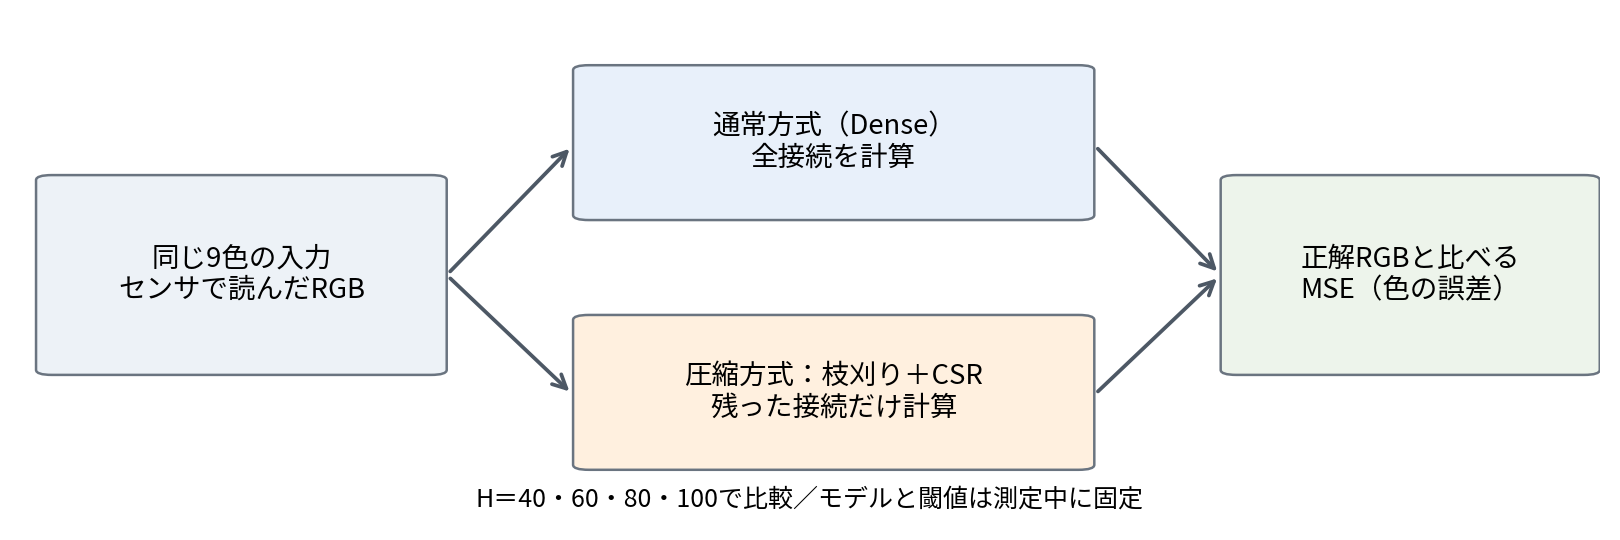
\includegraphics[width=0.95\textwidth,height=\textheight]{../figures/comparison_flow.png}

通常方式をDense、小さい重みを0にする枝刈りと、0を省いて保存するCSRを組み合わせた方式を圧縮方式と呼んだ。同じ読取データを両方式へ渡して比べた。

\begin{longtable}[]{@{}
  >{\raggedright\arraybackslash}p{(\columnwidth - 2\tabcolsep) * \real{0.5000}}
  >{\raggedright\arraybackslash}p{(\columnwidth - 2\tabcolsep) * \real{0.5000}}@{}}
\toprule\noalign{}
\begin{minipage}[b]{\linewidth}\raggedright
数字
\end{minipage} & \begin{minipage}[b]{\linewidth}\raggedright
自分の実験では何を意味するか
\end{minipage} \\
\midrule\noalign{}
\endhead
\bottomrule\noalign{}
\endlastfoot
9色 & 3×3の紙にある色の数 \\
135行 & 学習に使った入力と正解の組数。同じ色の繰返しを含む \\
H＝40・60・80・100 &
隠れ層それぞれの計算単位の数。色数や測定回数とは別 \\
8条件 & 4種類のH×Dense／枝刈り＋CSR \\
10回 & 9色を最後まで読み取った回数 \\
80個のMSE & 1回から8条件の結果が出るため、8×10個 \\
\end{longtable}

\textbf{PCの役割}は学習・枝刈り・CSRの準備である。\textbf{Arduinoの役割}は完成した重みを使って色を補正すること。学習した数値は.hファイルに保存した。

結論は、\textbf{容量と計算時間は減ったが、圧縮後の色の誤差は増えた}というもの。この理由を、次のページから順に読む。

\newpage

\section{2．センサの値をどうやって色に変えたか}\label{ux30bbux30f3ux30b5ux306eux5024ux3092ux3069ux3046ux3084ux3063ux3066ux8272ux306bux5909ux3048ux305fux304b}

\subsection{黒と白を登録した理由}\label{ux9ed2ux3068ux767dux3092ux767bux9332ux3057ux305fux7406ux7531}

黒と白を基準にして、各RGB成分の入力をそろえた。これを校正と正規化という。

\[\text{入力}=\frac{\text{読取値}-\text{黒の値}}{\text{白の値}-\text{黒の値}}\]

実際の1回目の赤成分では、黒9.8、白186.4、読取値137.5だったので、

\[\frac{137.5-9.8}{186.4-9.8}\approx0.7231\]

となる。ログのNN入力R＝0.7231はこの値である。黒の基準は0、白の基準は1になる。範囲外の値を0〜1へ収める処理がクリップである。

\subsection{Denseの計算は「掛けて足す」の繰返し}\label{denseux306eux8a08ux7b97ux306fux639bux3051ux3066ux8db3ux3059ux306eux7e70ux8fd4ux3057}

構造は「RGBの3入力→H個の計算→H個の計算→RGBの3出力」である。途中の2段が隠れ層で、H40なら各段に40個の計算単位がある。

1つの計算単位がすることは、\(z=w_RR+w_GG+w_BB+b\)。入力に掛ける係数wが重み、最後に足す調整値bがバイアスである。

実際のコードから、最初の段の1計算単位分を抜き出すと次のようになる。rは計算単位の番号、cはRGBの番号である。

\begin{Shaded}
\begin{Highlighting}[]
\DataTypeTok{float}\NormalTok{ value}\OperatorTok{=}\NormalTok{m}\OperatorTok{.}\NormalTok{b1}\OperatorTok{[}\NormalTok{r}\OperatorTok{];}
\ControlFlowTok{for}\OperatorTok{(}\DataTypeTok{int}\NormalTok{ c}\OperatorTok{=}\DecValTok{0}\OperatorTok{;}\NormalTok{c}\OperatorTok{\textless{}}\DecValTok{3}\OperatorTok{;}\NormalTok{c}\OperatorTok{++)}\NormalTok{ value}\OperatorTok{+=}\NormalTok{m}\OperatorTok{.}\NormalTok{w1}\OperatorTok{[}\NormalTok{r}\OperatorTok{*}\DecValTok{3}\OperatorTok{+}\NormalTok{c}\OperatorTok{]*}\NormalTok{input}\OperatorTok{[}\NormalTok{c}\OperatorTok{];}
\NormalTok{layer1}\OperatorTok{[}\NormalTok{r}\OperatorTok{]=}\NormalTok{value}\OperatorTok{\textgreater{}}\FloatTok{0.0}\BuiltInTok{f}\OperatorTok{?}\NormalTok{value}\OperatorTok{:}\FloatTok{0.0}\BuiltInTok{f}\OperatorTok{;}
\end{Highlighting}
\end{Shaded}

バイアスから合計を始め、RGBそれぞれに重みを掛けて足す。最後の行は「正ならそのまま、負なら0」にするReLUである。\texttt{r*3+c}は、並べて保存した重みの使う場所を指定する。

レポートの式
\(\boldsymbol h_1=\operatorname{ReLU}(W_1\boldsymbol x+\boldsymbol b_1)\)
は、この処理を全計算単位についてまとめて書いたもの。入力xから途中の結果hを作り、次の段へ渡す。最後に得た3出力を0〜1へ収め、255倍して四捨五入すると、PPMの整数RGBになる。

\newpage

\section{3．学習の式とL1正則化は何をしているか}\label{ux5b66ux7fd2ux306eux5f0fux3068l1ux6b63ux5247ux5316ux306fux4f55ux3092ux3057ux3066ux3044ux308bux304b}

学習は、予測した色を正解へ近づけるように重みを更新する作業である。PCで、135行を使い、V9の重みから40,000回の更新を行った。3×3の正解画像にはresult.ppmを使用した。

\textbf{学習式の意味は「色の誤差＋重みを大きくしすぎない罰則」である。}
実際の式は次のとおり。

\[
\mathcal L=\frac{1}{\sum_i a_i}\sum_i\frac{a_i}{3}\sum_{c\in\{R,G,B\}}
\ell_\beta(\widehat y_{i,c}-t_{i,c})
+10^{-6}\sum_{\ell=1}^{3}\sum_{j,k}|(W_\ell)_{jk}|.
\]

\begin{longtable}[]{@{}ll@{}}
\toprule\noalign{}
記号 & 意味 \\
\midrule\noalign{}
\endhead
\bottomrule\noalign{}
\endlastfoot
i、c & 学習行の番号とRGBの成分 \\
\(\widehat y\)、t & 予測値と正解。学習ではRGBを255で割った尺度を使う \\
\(a_i\) & 学習行ごとの重要度。ネットワーク内の重みWとは別 \\
\(\sum\) & 指定範囲の値を全て足す記号 \\
\(\ell\)、j、k & 層の番号と、その重みの表の中の位置 \\
\end{longtable}

前半は色の誤差を、各行の重要度に従って平均する部分。誤差にはSmooth
L1を使った。

\[\ell_\beta(e)=\begin{cases}e^2/(2\beta)&(|e|<\beta),\\ |e|-\beta/2&(|e|\geq\beta),\end{cases}\quad\beta=0.05\]

eは予測と正解の差。小さい誤差では二乗、大きい誤差では直線的に増える。一部の大きな誤差だけに学習が強く引っ張られることを抑えるために使った。

後半がL1正則化で、全3層の重みの絶対値を足し、\(10^{-6}\)倍して加える。外側の\(\sum\)で層、内側の\(\sum\)で各重みを足す。重みが大きいほど罰則が増えるため、小さい重みを作る方向にも更新される。バイアスにはこの罰則を付けない。

Pythonでは、\texttt{loss\_rows}でRGB誤差を求め、\texttt{(loss\_rows*weights).sum()/weights.sum()}で重要度付き平均にし、L1項を加えた。\texttt{loss.backward()}で更新方向を計算し、\texttt{optimizer.step()}で重みを更新した。

\textbf{beta＝0.05は学習式の切替値で、枝刈りの閾値とは別。学習時の損失も、結果表のMSEとは別の値である。}

\newpage

\section{4．枝刈りとCSRは、それぞれ何をしたか}\label{ux679dux5208ux308aux3068csrux306fux305dux308cux305eux308cux4f55ux3092ux3057ux305fux304b}

\subsection{枝刈り＝小さい重みを0にする}\label{ux679dux5208ux308aux5c0fux3055ux3044ux91cdux307fux30920ux306bux3059ux308b}

\[|w|<\tau\quad\Rightarrow\quad w=0\]

閾値\(\tau\)は重みを残す境目。H60では約0.0543だった。例えば0.03や−0.03は0になり、0.2や−0.2は残る。符号ではなく絶対値で判断し、バイアスは変えない。

候補は学習済み重みの値から作った。別の8×8チャートの128入力で、MSE増加5\%以下かつ容量が小さくなるものを残し、学習内9入力でMSE300以下も満たす候補から最小容量を選んだ。新規10回の測定中は固定した。

\subsection{CSR＝0を省き、残した値と位置を保存する}\label{csr0ux3092ux7701ux304dux6b8bux3057ux305fux5024ux3068ux4f4dux7f6eux3092ux4fddux5b58ux3059ux308b}

説明用の小さな例を考える。これは実測の重みではない。

\begin{Shaded}
\begin{Highlighting}[]
\NormalTok{元の表       [ 0,    0.5, 0   ]}
\NormalTok{             [{-}0.2,  0,   0.1 ]}
\NormalTok{values  = [0.5, {-}0.2, 0.1]   ← 0以外の値}
\NormalTok{columns = [1,    0,   2  ]   ← 元の列番号（0始まり）}
\NormalTok{rows    = [0,    1,   3  ]   ← 各行の開始位置と終端}
\end{Highlighting}
\end{Shaded}

rowsの0〜1の手前が1行目、1〜3の手前が2行目なので、1行目はvaluesの0番だけ、2行目は1番と2番を使う。入力\((x_0,x_1,x_2)\)に対し、\(0.5x_1\)と\(-0.2x_0+0.1x_2\)を計算できる。

実際のArduino関数は次のとおり。\texttt{layer.col}がcolumns、\texttt{layer.row}がrowsである。

\begin{Shaded}
\begin{Highlighting}[]
\DataTypeTok{void}\NormalTok{ sparseLayer}\OperatorTok{(}\AttributeTok{const}\NormalTok{ comparison\_models}\OperatorTok{::}\NormalTok{SparseLayer }\OperatorTok{\&}\NormalTok{layer}\OperatorTok{,}\AttributeTok{const} \DataTypeTok{float} \OperatorTok{*}\NormalTok{input}\OperatorTok{,}\DataTypeTok{float} \OperatorTok{*}\NormalTok{output}\OperatorTok{,}\DataTypeTok{bool}\NormalTok{ relu}\OperatorTok{)} \OperatorTok{\{}
  \ControlFlowTok{for}\OperatorTok{(}\DataTypeTok{int}\NormalTok{ r}\OperatorTok{=}\DecValTok{0}\OperatorTok{;}\NormalTok{r}\OperatorTok{\textless{}}\NormalTok{layer}\OperatorTok{.}\NormalTok{rows}\OperatorTok{;}\NormalTok{r}\OperatorTok{++)} \OperatorTok{\{}
    \DataTypeTok{float}\NormalTok{ value}\OperatorTok{=}\NormalTok{layer}\OperatorTok{.}\NormalTok{bias}\OperatorTok{[}\NormalTok{r}\OperatorTok{];}
    \ControlFlowTok{for}\OperatorTok{(}\DataTypeTok{uint16\_t}\NormalTok{ k}\OperatorTok{=}\NormalTok{layer}\OperatorTok{.}\NormalTok{row}\OperatorTok{[}\NormalTok{r}\OperatorTok{];}\NormalTok{k}\OperatorTok{\textless{}}\NormalTok{layer}\OperatorTok{.}\NormalTok{row}\OperatorTok{[}\NormalTok{r}\OperatorTok{+}\DecValTok{1}\OperatorTok{];}\NormalTok{k}\OperatorTok{++)}\NormalTok{ value}\OperatorTok{+=}\NormalTok{layer}\OperatorTok{.}\NormalTok{values}\OperatorTok{[}\NormalTok{k}\OperatorTok{]*}\NormalTok{input}\OperatorTok{[}\NormalTok{layer}\OperatorTok{.}\NormalTok{col}\OperatorTok{[}\NormalTok{k}\OperatorTok{]];}
\NormalTok{    output}\OperatorTok{[}\NormalTok{r}\OperatorTok{]=(}\NormalTok{relu }\OperatorTok{\&\&}\NormalTok{ value}\OperatorTok{\textless{}}\DecValTok{0}\OperatorTok{)?}\DecValTok{0}\OperatorTok{:}\NormalTok{value}\OperatorTok{;}
  \OperatorTok{\}}
\OperatorTok{\}}
\end{Highlighting}
\end{Shaded}

rは行、kは保存した重みの番号。バイアスを用意し、その行に残った重みだけを対応する入力へ掛けて足す。ReLUは隠れ層だけで使う。

\textbf{CSR変換の正しさ}は、枝刈り後の重みを通常配列で計算した結果と照合した。\textbf{圧縮の精度への影響}は、枝刈り前のDenseと比較した。変換が正しくても、枝刈りで色の誤差は増える場合がある。

\newpage

\section{5．MSEと「10回平均」「10回目」の違い}\label{mseux306810ux56deux5e73ux574710ux56deux76eeux306eux9055ux3044}

MSEは、補正後の色yと先生指定画像の正解tのずれ。9色×RGBの3成分＝27個を比べる。

\[\mathrm{MSE}=\frac1{27}\sum_{i=1}^{9}\sum_{c\in\{R,G,B\}}(y_{i,c}-t_{i,c})^2\]

27個それぞれの差を二乗して足し、27で割る。説明用に、全ての差が10ならMSEは100になる。0なら全て一致し、小さいほど正確である。

\textbf{レポートの結果表は、次の10回平均を使っている。}
MSEは小数第2位まで表示し、第3位以降を切り捨てる。平均は切り捨て前の値で計算する。

\begin{longtable}[]{@{}lrr@{}}
\toprule\noalign{}
H & Dense平均MSE & 枝刈り＋CSR平均MSE \\
\midrule\noalign{}
\endhead
\bottomrule\noalign{}
\endlastfoot
40 & 319.56 & 452.04 \\
60 & 238.33 & 493.51 \\
80 & 231.68 & 465.72 \\
100 & 260.42 & 651.92 \\
\end{longtable}

例えばH60のDenseは、10回目の画像のMSEが2.33だが、10回平均は238.33である。

\begin{longtable}[]{@{}
  >{\centering\arraybackslash}p{(\columnwidth - 4\tabcolsep) * \real{0.3333}}
  >{\centering\arraybackslash}p{(\columnwidth - 4\tabcolsep) * \real{0.3333}}
  >{\centering\arraybackslash}p{(\columnwidth - 4\tabcolsep) * \real{0.3333}}@{}}
\toprule\noalign{}
\begin{minipage}[b]{\linewidth}\centering
先生指定の正解
\end{minipage} & \begin{minipage}[b]{\linewidth}\centering
H60 Dense・2回目
\end{minipage} & \begin{minipage}[b]{\linewidth}\centering
H60 Dense・10回目
\end{minipage} \\
\midrule\noalign{}
\endhead
\bottomrule\noalign{}
\endlastfoot

\includegraphics[width=39mm,height=\textheight]{../color_images/reference.png}
&
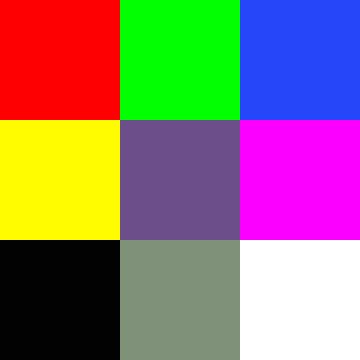
\includegraphics[width=39mm,height=\textheight]{../color_images/capture_02/h60_dense.png}
&

\includegraphics[width=39mm,height=\textheight]{../color_images/capture_10/h60_dense.png} \\
比較の基準 & MSE 2339.37 & MSE 2.33 \\
\end{longtable}

2回目の大きな誤差も含めた全10回の平均なので、平均は高くなる。操作ミスの申告がなかったため、その回も含めた。平均値に対応する実測画像が1枚あるわけではなく、10回目の画像へ平均MSEを付けて、その1枚の誤差として扱うことはできない。

平均は
\(\overline m=(m_1+\cdots+m_{10})/10\)。SD（標本標準偏差）は各回がどれだけばらついたかを表す。平均が小さくても、SDや最大値が大きければ、毎回安定して正確とはいえない。

\newpage

\section{6．容量の式と、Flash・RAMの違い}\label{ux5bb9ux91cfux306eux5f0fux3068flashramux306eux9055ux3044}

\subsection{DenseとCSRの容量を手計算する}\label{denseux3068csrux306eux5bb9ux91cfux3092ux624bux8a08ux7b97ux3059ux308b}

FP32は数値1個に4 byte使う。Denseの重み数は \(3H+H^2+3H\)、バイアス数は
\(H+H+3\)なので、

\[B_{\mathrm{Dense}}=4(H^2+8H+3)\]

H60なら重み3,960個、バイアス123個で、\(4(3,960+123)=16,332\)
byteになる。

CSRでは、残った重みK個が4K byte、列番号がK byte、行の開始位置が
\(2(2H+6)\) byte、バイアスが \(4(2H+3)\) byteになる。

\[B_{\mathrm{CSR}}=4K+K+2(2H+6)+4(2H+3)=5K+12H+24\]

H60はK＝1,141なので、\(4,564+1,141+252+492=6,449\) byteである。削減率は
\(100(1-6,449/16,332)=60.51\%\)。位置情報にも容量が必要なので、重みがあまり減らない場合はCSRでも小さくならない。

\subsection{モデルだけの容量と、プログラム全体を分ける}\label{ux30e2ux30c7ux30ebux3060ux3051ux306eux5bb9ux91cfux3068ux30d7ux30edux30b0ux30e9ux30e0ux5168ux4f53ux3092ux5206ux3051ux308b}

Flashはプログラム等を保存する領域、RAMは動作中の作業領域である。1モデルずつ入れたプログラム全体のFlashは次のようになった。

\begin{longtable}[]{@{}lrrr@{}}
\toprule\noalign{}
H & Dense Flash byte & CSR Flash byte & 削減率 \\
\midrule\noalign{}
\endhead
\bottomrule\noalign{}
\endlastfoot
40 & 60,852 & 56,020 & 7.94\% \\
60 & 69,492 & 59,612 & 14.22\% \\
80 & 81,348 & 62,396 & 23.30\% \\
100 & 96,388 & 66,260 & 31.26\% \\
\end{longtable}

H60のモデル配列は60.51\%減ったが、Flash全体は14.22\%の削減だった。Arduinoの基本処理など、両方式で共通の部分が残るためである。

静的RAMは全8条件で6,764 byteと同じ。32,768−6,764＝26,004
byteは静的割当後の残りであり、ローカル変数が実際に使った量ではない。

関数内で一時的に使う領域がスタック。元の中間配列はfloat{[}100{]}を2本で、宣言上800
byteだが、他の処理もあるため最大使用量は別に測る必要がある。今回は未測定である。

\newpage

\section{7．速度のコードと、測った時間の範囲}\label{ux901fux5ea6ux306eux30b3ux30fcux30c9ux3068ux6e2cux3063ux305fux6642ux9593ux306eux7bc4ux56f2}

使ったのは、保存済みの実測9入力をArduinoへ繰り返し入れる方法。新たに紙を読む時間ではなく、色の補正を計算する区間を測った。

実際の関数は次のとおり。\texttt{micros()}は動作開始からの時間をµsで読み、1
µsは100万分の1秒である。

\begin{Shaded}
\begin{Highlighting}[]
\DataTypeTok{uint32\_t}\NormalTok{ timeModel}\OperatorTok{(}\DataTypeTok{int}\NormalTok{ model}\OperatorTok{,}\DataTypeTok{int}\NormalTok{ group}\OperatorTok{,}\DataTypeTok{double} \OperatorTok{\&}\NormalTok{checksum}\OperatorTok{)} \OperatorTok{\{}
  \DataTypeTok{float}\NormalTok{ output}\OperatorTok{[}\DecValTok{3}\OperatorTok{];}\NormalTok{checksum}\OperatorTok{=}\DecValTok{0}\OperatorTok{;}
  \DataTypeTok{uint32\_t}\NormalTok{ begin}\OperatorTok{=}\KeywordTok{static\_cast}\OperatorTok{\textless{}}\DataTypeTok{uint32\_t}\OperatorTok{\textgreater{}(}\NormalTok{micros}\OperatorTok{());}
  \ControlFlowTok{for}\OperatorTok{(}\DataTypeTok{int}\NormalTok{ call}\OperatorTok{=}\DecValTok{0}\OperatorTok{;}\NormalTok{call}\OperatorTok{\textless{}}\DecValTok{100}\OperatorTok{;}\NormalTok{call}\OperatorTok{++)} \OperatorTok{\{}
    \DataTypeTok{int}\NormalTok{ input}\OperatorTok{=(}\NormalTok{group}\OperatorTok{*}\DecValTok{100}\OperatorTok{+}\NormalTok{call}\OperatorTok{)\%}\NormalTok{comparison\_models}\OperatorTok{::}\NormalTok{BENCHMARK\_INPUT\_COUNT}\OperatorTok{;}
\NormalTok{    comparison\_models}\OperatorTok{::}\NormalTok{predict}\OperatorTok{(}\NormalTok{model}\OperatorTok{,}\NormalTok{comparison\_models}\OperatorTok{::}\NormalTok{BENCHMARK\_INPUTS}\OperatorTok{[}\NormalTok{input}\OperatorTok{],}\NormalTok{output}\OperatorTok{);}
\NormalTok{    checksum}\OperatorTok{+=}\NormalTok{output}\OperatorTok{[}\DecValTok{0}\OperatorTok{]+}\NormalTok{output}\OperatorTok{[}\DecValTok{1}\OperatorTok{]+}\NormalTok{output}\OperatorTok{[}\DecValTok{2}\OperatorTok{];}
  \OperatorTok{\}}
  \ControlFlowTok{return} \KeywordTok{static\_cast}\OperatorTok{\textless{}}\DataTypeTok{uint32\_t}\OperatorTok{\textgreater{}(}\NormalTok{micros}\OperatorTok{()){-}}\NormalTok{begin}\OperatorTok{;}
\OperatorTok{\}}
\end{Highlighting}
\end{Shaded}

\begin{longtable}[]{@{}ll@{}}
\toprule\noalign{}
コード & していること \\
\midrule\noalign{}
\endhead
\bottomrule\noalign{}
\endlastfoot
\texttt{begin=micros()} & 開始時刻を保存する \\
\texttt{call\textless{}100} & 100回まとめて計算する \\
\texttt{...\ \%\ BENCHMARK\_INPUT\_COUNT} &
保存した9入力を順に繰り返す \\
\texttt{predict(...)} & 指定モデルで色を補正する \\
\texttt{checksum+=...} & 出力を足し、計算結果が使われるようにする \\
\texttt{micros()-begin} & 100推論分の経過時間を返す \\
\end{longtable}

その時間を100で割って1推論当たりの値にした。各モデルは最初に10回動かしてから、100推論を5組計った。Dense先行とCSR先行を交互にした。

\begin{longtable}[]{@{}lrrr@{}}
\toprule\noalign{}
H & Dense µs/推論 & CSR µs/推論 & 短縮率 \\
\midrule\noalign{}
\endhead
\bottomrule\noalign{}
\endlastfoot
40 & 465.262 & 305.834 & 34.27\% \\
60 & 945.648 & 671.674 & 28.97\% \\
80 & 1593.368 & 956.212 & 39.99\% \\
100 & 2408.160 & 1348.392 & 44.01\% \\
\end{longtable}

H60の945.648 µsは約0.000946秒、671.674
µsは約0.000672秒。計算時間は28.97\%短くなった。

紙を動かす時間、センサ読取、シリアル出力、MSE計算は計時区間へ含めていない。一方、入力選択と出力の合計は含まれる。したがって、紙の読取全体や推論関数だけを単独で測った時間とは区別する。

\newpage

\section{8．結果をどう説明すればよいか}\label{ux7d50ux679cux3092ux3069ux3046ux8aacux660eux3059ux308cux3070ux3088ux3044ux304b}

\subsection{H60の1組で、指標をつなげて考える}\label{h60ux306e1ux7d44ux3067ux6307ux6a19ux3092ux3064ux306aux3052ux3066ux8003ux3048ux308b}

\begin{longtable}[]{@{}lrr@{}}
\toprule\noalign{}
指標 & Dense & 枝刈り＋CSR \\
\midrule\noalign{}
\endhead
\bottomrule\noalign{}
\endlastfoot
新規10回の平均MSE & 238.33 & 493.51 \\
モデル配列容量 byte & 16,332 & 6,449 \\
プログラム全体のFlash byte & 69,492 & 59,612 \\
静的RAM byte & 6,764 & 6,764 \\
計算時間 µs/推論 & 945.648 & 671.674 \\
\end{longtable}

\textbf{小さくなり、速くなった。しかし、色の誤差は増えた。}
全4種類のHでも、圧縮後の平均MSEは増えた。MSE増加5\%以下と、圧縮方式の10回平均MSE300以下という目標は達成しなかった。

\subsection{自分の言葉で説明する例}\label{ux81eaux5206ux306eux8a00ux8449ux3067ux8aacux660eux3059ux308bux4f8b}

「色補正ニューラルネットワークを、通常のDenseと枝刈り＋CSRで比較しました。小さい重みを0にし、残った値と位置だけを保存して計算を減らしました。40・60・80・100次元で、同じ9色の入力を両方式に使って10回測りました。モデルの容量と計算時間は減りましたが、圧縮後のMSEが増えたため、精度維持は達成できませんでした。」

\subsection{混同しやすい点}\label{ux6df7ux540cux3057ux3084ux3059ux3044ux70b9}

\textbf{PASSの意味。}
固定入力でPCとArduinoの計算が一致し、CSRの位置情報が正しいことを確認した。色が正解に近いかは別にMSEで判断するので、PASSでもMSEは悪くなり得る。

\textbf{測定した範囲。}
新規入力は学習や閾値選択に加えていないが、紙の色は学習にも使ったもの。学習に使っていない別の紙での最終確認は未実施である。

\textbf{まだ測っていないもの。}
H50・H200、各方式が何次元まで載るか、実行時スタックの最大量は未測定。今後は削る量の見直し、枝刈り後の追加学習、入力変動の確認、別の紙での評価が候補になる。

提出用の本文は \href{../report.pdf}{report.pdf}、色画像は
\href{../color_images/README.md}{color\_images}。このガイドは、その本文・保存済みコード・実測CSVの内容を説明したもので、測定値やモデルを変更していない。

\end{document}
